\newpage

\section{Quartz Scheduler}
Pro synchronizaci dat a~spouštění úloh v~určitých intervalech je použit \texttt{Quartz Scheduler}.
Ten je přímo integrován do frameworku Spring Boot jako součást jedné z~jeho knihoven.
Samotný scheduler se spouští při startu aplikace.
Po startu aplikace se spustí úlohy neboli \textit{Jobs}.

\subsection{Jobs}
\textit{Joby} jsou úlohy, které se spouštějí v~určitých intervalech nebo na základě určité události.
V~našem případě se jedná o~3 úlohy:
\begin{itemize}
    \item \texttt{InitStatAzZsj} -- inicializace základních územních prvků a~krajů.
    \item \texttt{InitRegion} -- inicializace regionů.
    \item \texttt{Additions} -- přírůstková data, která se stahují každý den.
\end{itemize}

\subsubsection*{InitStatAzZsj}
Tato úloha se spouští při startu aplikace a~je zodpovědná za inicializaci základních územních prvků a~krajů.
Pokud je v~konfiguraci nastaveno přeskočení inicializace těchto prvků, úloha se neprovede.
Úloha nejprve stáhne data o~základních územních prvcích a~krajích z~API RÚIAN za poslední měsíc.
Následně se soubor zpracuje a~data se uloží do databáze.

\subsubsection*{InitRegion}
Tato úloha se spouští jako druhá, bezprostředně po dokončení úlohy \texttt{InitStatAzZsj}.
Pokud je v~konfiguraci nastaveno přeskočení inicializace regionů, tato úloha se přeskočí.
Úloha ze zadané konfigurace načte všechny kraje, které byly uvedeny.
Každý kraj má přiřazen seznam obcí, které se postupně stahují z~API RÚIAN, zpracují a~uloží do databáze.

\subsubsection*{Additions}
Tato úloha se spouští na základě nastavení v~konfiguračním souboru nebo po dokončení úlohy \texttt{InitRegion}.
Každý den je na API RÚIAN vytvořen nový soubor s~přírůstkovými daty za poslední den.
Úloha tento soubor stáhne, zpracuje a~uloží do databáze.
Poté čeká na další spuštění podle časového nastavení v~konfiguraci.

\subsection{Triggers}
\textit{Triggers} jsou spouštěče, které určují, kdy se má daný \texttt{job} spustit.
Jak bylo zmíněno výše, úlohy \texttt{InitStatAzZsj} a~\texttt{InitRegion} se spouštějí jednorázově při startu aplikace a~navazují na sebe.
Úloha \texttt{Additions} se spouští pravidelně podle nastavení v~konfiguračním souboru.
Konkrétně je čas spuštění definován v~cron formátu popsán v~sekci \ref{sec:cron_format}.

\subsection{Zajištění správného pořadí}
Je důležité zajistit, aby se úlohy spouštěly ve~správném pořadí.
Kdyby se spustila úloha \texttt{Additions} před úlohou \texttt{InitRegion}, 
mohlo by dojít k~problémům s~neexistujícími daty.
Tomu se předejde vytvořením závislostí mezi joby.
Pořadí spuštění jobů je znázorněno na obrázku \ref{fig:jobs_scheduled}.

\begin{figure}[!h]
    \caption{Pořadí jobů}
    \label{fig:jobs_scheduled}
    \centering
    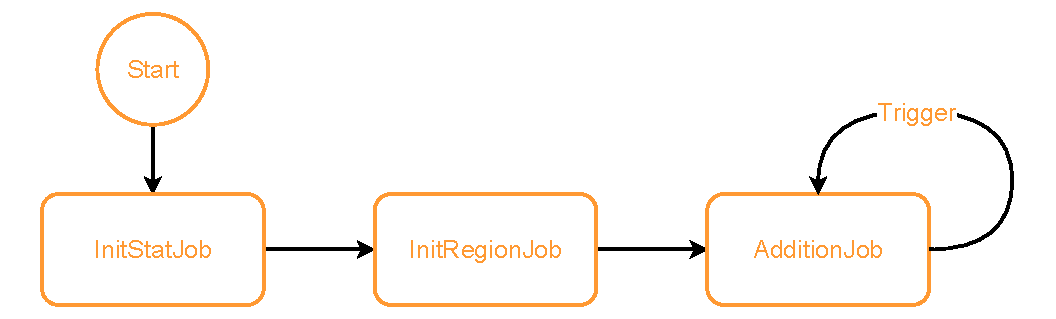
\includegraphics[width=\textwidth]{figures/jobs_scheduled.pdf}
\end{figure}

Při startu aplikace se spustí job \texttt{InitStatAzZsj}, až úspěšně skončí,
spustí se job \texttt{InitRegion}. Pokud je v konfiguraci nastaveno, že se job
přeskočí, tak se job stále provede a~dokončí jen bez zpracování dat.
Stejně to platí pro job \texttt{InitRegionJob}.
Problémem bylo, že job \texttt{InitStatAzZsj} a~\texttt{Additions}
se spouštěly vždy při startu aplikace, protože měly trigger pro start.
Ovšem job \texttt{Additions} se má spustit až po úspěšném dokončení jobu
\texttt{InitRegion}. Tento problém byl vyřešen pomocí \textbf{Semaforu}.
Konkrétně byl použit \texttt{Semaphore} z~balíčku \texttt{java.util.concurrent}.
Vzhledem k~tomu, že Quartz Scheduler má pro každý job vlastní vlákno,
je možné použít \texttt{Semaphore} pro zajištění, že se job \texttt{Additions}
může spustit až po úspěšném dokončení jobu \texttt{InitRegion}.

Semafor je inicializován na hodnotu 0, což znamená, že job \texttt{Additions}
se nemůže spustit, dokud není semafor uvolněn. Ten je uvolněn následně na konci
jobu \texttt{InitRegion}. Jakmile se job \texttt{Additions} spustí poprvé, je pak
opakovaně spouštěn podle nastavení cron v~konfiguračním souboru.

\subsubsection*{Semafor}
Semafor je synchronizační primitivum, které umožňuje řídit přístup
k~sdíleným prostředkům v~multithreadovém prostředí.
Semafor může být binární (0 nebo 1) nebo počítací (libovolné celé číslo).
Následně má dvě hlavní operace:
\begin{itemize}
    \item \texttt{V()} -- uvolnění semaforu, zvýšení hodnoty semaforu o~1.
    \item \texttt{P()} -- zablokování semaforu, snížení hodnoty semaforu o~1, pokud je hodnota semaforu 0, vlákno se zablokuje a~čeká na uvolnění semaforu.
\end{itemize}

Tyto dvě operace jsou atomické, což znamená, že jsou prováděny jako jedna operace a~nelze je přerušit.
V Javě je semafor implementován pomocí třídy \texttt{Semaphore} z~balíčku \texttt{java.util.concurrent}.
P a V operace jsou implementovány jako metody \texttt{acquire()} a~\texttt{release()}.
Více o semaforech a~jeho použití je popsáno v~\cite{pesicka_semafor}.


